\Chapter{GENERAL DISCUSSIONS}\label{sec:discussions}

\textit{
    The developments presented in this thesis introduce alternative numerical approaches at three distinct stages of the ice-accretion framework: Eulerian and Lagrangian formulations for droplet impingement, algebraic surface displacement and level-set methods for geometry evolution, and body-fitted and immersed-boundary approaches for the treatment of the evolving geometry. Each alternative introduces different compromises between computational efficiency, numerical robustness, implementation complexity, and modeling capabilities. This chapter discusses these trade-offs collectively, with particular emphasis on how the appropriate methodology depends on the complexity and objectives of the icing simulation.
    }

\subsection{Eulerian and Lagrangian Droplet Impingement}

The first two Ice Prediction Workshops primarily focused on assessing the ability of numerical icing tools to reproduce experimental ice shapes. Although the final ice geometry provides an important validation metric, ice accretion results from the successive coupling of the different modules discussed throughout this thesis. Agreement or disagreement in the final ice shape cannot therefore necessarily be attributed to a particular component of the icing framework. The recent third Ice Prediction Workshop (IPW3) consequently placed greater emphasis on the verification and validation of the individual components of the icing framework. For droplet impingement, one of the questions considered was whether the Eulerian and Lagrangian formulations converge toward consistent predictions despite their different descriptions of the dispersed phase.

The IPW3 test cases included the NACA0012 and the ONERA M6 wing, both considered in a 3D setup. The corresponding reference conditions prescribed for the workshop are summarized in Table~\ref{tab:droplet_benchmark_conditions}. In the present section, the NACA0012 configuration is used to compare the integrated collected-water mass predicted by the Eulerian and Lagrangian formulations across successive grid refinements. The ONERA M6 configuration provides a complementary benchmark for assessing the computational performance of both formulations and the time required to obtain the corresponding impingement solutions.

\begin{table}[htbp]
\centering
\caption{Reference conditions for the IPW3 droplet-impingement benchmark cases.}
\label{tab:droplet_benchmark_conditions}
\begin{tabular}{lcc}
\hline
& NACA0012 & ONERA M6 \\
\hline
$M_\infty$             & 0.315            & 0.400 \\
$\alpha$ [$^\circ$]    & 4.0              & 2.0 \\
$Re$                   & $4.40\times10^6$ & $4.256\times10^6$ \\
LWC [g/m$^3$]          & 0.55             & 0.51 \\
MVD [$\mu$m]           & 20               & 20 \\
$c_\mathrm{ref}$ [m]   & 0.5334           & 0.801673 \\
\hline
\end{tabular}
\end{table}

\begin{table}[htbp]
\centering
\caption{NACA0012 grid hierarchy.}
\label{tab:naca_grid_hierarchy}
\begin{tabular}{cc}
\hline
Grid level & Elements \\
\hline
L4 & 5,861,000 \\
L3 & 11,079,000 \\
L2 & 26,988,000 \\
L1 & 59,863,000 \\
\hline
\end{tabular}
\end{table}

\begin{figure}[htbp]
\centering
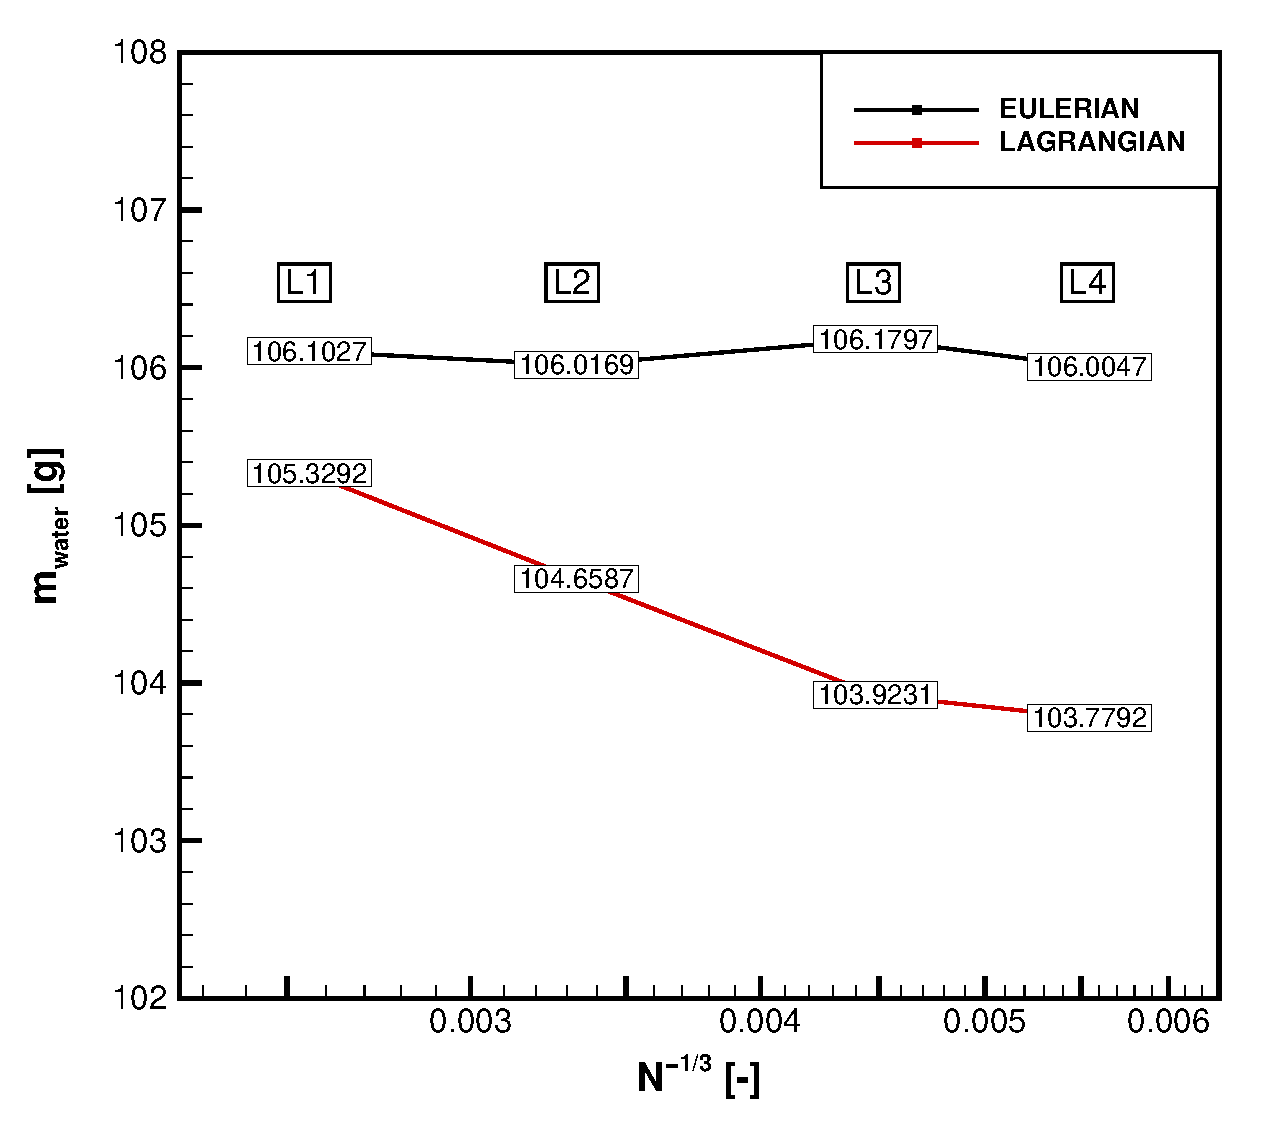
\includegraphics[width=0.7\textwidth]
{FIGURES/DISCUSSIONS/NACA0012_IPW3_EUL_VS_LAG.eps}
\caption{Spatial convergence of the integrated collected-water mass obtained with the Eulerian and Lagrangian droplet formulations for the NACA0012 IPW3 configuration using the MVD of $20~\mu$m.}
\label{fig:naca_eul_lag_convergence}
\end{figure}

Figure~\ref{fig:naca_eul_lag_convergence} compares the integrated collected-water mass predicted by the Eulerian and Lagrangian formulations over the grid sequence summarized in Table~\ref{tab:naca_grid_hierarchy}. Results are shown for droplets corresponding to the MVD of $20~\mu$m. The difference between the two formulations remains below $2\%$ over the complete grid sequence and systematically decreases with spatial refinement. The figure also highlights a greater sensitivity of the Lagrangian prediction to the underlying volume-mesh resolution. This behavior can be attributed in part to the repeated interpolation of the carrier-flow quantities along a large number of droplet trajectories following different paths through the computational domain. Consequently, changes in the spatial resolution of the underlying flow field can influence the integrated collected-water mass through the trajectory calculations. In contrast, the Eulerian droplet equations are solved directly on the volume mesh using the local flow solution, resulting in considerably less variation of the integrated collected-water mass over the present grid sequence. Nonetheless, the Eulerian and Lagrangian formulations converge toward consistent integrated impingement predictions with spatial refinement, reaching a difference of $0.8\%$ on Level~1.

The computational performance of the two formulations is compared for the ONERA M6 configuration, with representative timings reported in Table~\ref{tab:m6_eul_lag_performance}. The Level~4 calculation was performed on a workstation equipped with an Intel Xeon w7-2595X processor with 26 physical cores. The Level~1 calculation was performed on 8 Trillium cluster compute nodes, each containing two AMD EPYC 9655 processors with 96 cores per socket, corresponding to 192 physical cores per node. The hardware information is provided for reference to distinguish between the shared-memory and distributed-memory calculations.

\begin{table}[htbp]
\centering
\caption{Representative computational performance of the Eulerian and Lagrangian droplet formulations for the ONERA M6 configuration.}
\label{tab:m6_eul_lag_performance}
\begin{tabular}{cccccc}
\hline
Grid &
Elements &
Eul. [s] &
Lag. [s] &
ETR* [\%] &
Hardware \\
\hline
L4 &
135,168 &
83.05 &
15.40 &
81.5 &
Xeon w7-2595X \\
L1 &
69,206,016 &
1501.81 &
1182.13 &
21.3 &
8 $\times$ 2 AMD EPYC 9655 \\
\hline
\end{tabular}

\begin{minipage}{\textwidth}
\raggedright
\footnotesize
\textit{Note:} ETR: execution-time reduction.
\end{minipage}

\end{table}

The Lagrangian formulation is particularly attractive when the computational mesh can be efficiently accessed within shared memory, allowing trajectories to traverse the domain without requiring remote access to flow and mesh data. For the ONERA M6 calculations reported here, the Lagrangian formulation reduces the execution time relative to the Eulerian formulation by $81.5\%$ on Level~4 and $21.3\%$ on Level~1. For the larger distributed-memory calculation, the required flow and mesh data are replicated across the compute nodes to minimize communication during trajectory integration. This replication represents a necessary trade-off: although it substantially reduces remote data accesses, it increases the memory requirements on each compute node and can become restrictive as the mesh size increases. In addition, the irregular memory-access patterns associated with trajectory tracking make the Lagrangian formulation more susceptible to memory-bandwidth limitations and cache misses as the number of concurrent trajectories increases. These effects reduce the computational advantage of the Lagrangian formulation on the Level~1 case despite limiting inter-node communication.

The Eulerian formulation naturally follows the spatial decomposition of the computational mesh, making its parallel execution relatively straightforward to configure. In contrast, the Lagrangian performance reported here was achieved after careful optimization of the adaptive seeding strategy, trajectory workload balancing, and execution configuration according to the underlying cluster architecture. Efficient Lagrangian simulations on large 3D problems therefore require greater implementation effort and knowledge of the computing environment, while the Eulerian formulation is generally easier to configure for distributed-memory calculations.

\subsection{Algebraic and Level-Set Ice Accretion}

Explicit algebraic surface displacement presents important limitations for 3D multilayer ice accretion as increasingly complex ice features develop. Figure~\ref{fig:algebraic_vs_levelset} compares the algebraic and level-set approaches under the same icing conditions and using the same number of accretion layers ($N_{\mathrm{layers}}=5$), such that the differences observed between the final geometries originate primarily from the geometry-evolution procedure. With the algebraic approach, successive displacement of the surface nodes causes the mesh to become increasingly susceptible to local folding and element entanglement. Extensive surface smoothing is therefore required between successive accretion steps to maintain a valid computational surface. Although this stabilizes the geometry-evolution procedure, it also progressively damps the smaller-scale ice features generated during the accretion process. This effect is clearly visible in Fig.~\ref{fig:algebraic_vs_levelset}, where the algebraic solution exhibits a considerably smoother and more uniform ice structure. In contrast, the level-set formulation allows the interface to evolve without being directly constrained by the connectivity of the previous surface mesh and requires little to no surface smoothing, thereby preserving substantially more of the 3D structures that develop during successive accretion layers.

\begin{figure}[htbp]
    \centering
    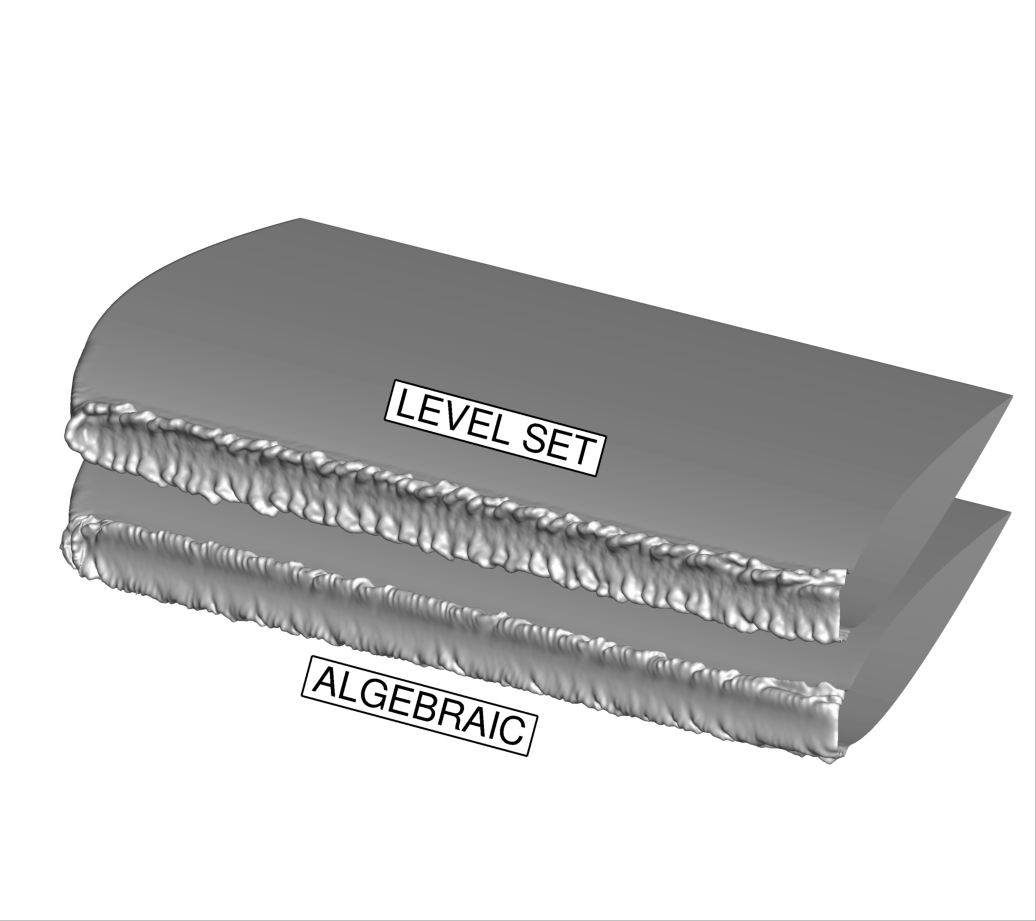
\includegraphics[trim={1cm 5cm .5cm 5cm}, clip,width=0.7\textwidth]{FIGURES/DISCUSSIONS/ALGEBRAIC_VS_LEVEL_SET.png}
    \caption{Comparison of algebraic and level-set ice shapes under identical icing conditions after five accretion layers.}
    \label{fig:algebraic_vs_levelset}
\end{figure}

This difference has implications beyond the prediction of an individual ice shape. In practice, the robustness of the geometry-evolution procedure determines which numerical experiments can be performed reliably. With algebraic displacement, increasingly complex geometries or a larger number of accretion layers can require case-dependent smoothing and remeshing parameters, while severe surface distortion may still lead to failure before completion of the simulation. Consequently, the geometry-update procedure itself can become a limiting factor when attempting to investigate the sensitivity of the complete icing framework to physical and numerical parameters.

The level-set methodology substantially reduces this limitation and therefore provides a more suitable framework for systematic investigations of 3D multilayer ice accretion. Once the geometry evolution is sufficiently robust, different icing conditions, droplet-size distributions, spatial resolutions, and numbers of accretion layers can be investigated without the same concern that the evolving surface will fold onto itself or cause the simulation to fail midway through the accretion sequence. This capability is particularly important because the resulting 3D ice morphology can exhibit a strong sensitivity to these parameters. As illustrated in Fig.~\ref{fig:levelset_parametric_shapes}, different structures can emerge along the iced leading edge depending on the droplet-size distribution, the number of accretion layers, and the spatial resolution used to represent the evolving interface. The level-set methodology therefore provides not only a more robust geometry-evolution technique, but also an enabling tool for exploring the underlying numerical and physical mechanisms governing the development of complex 3D ice structures, such as scallop formation.

\begin{figure}[htbp]
    \centering
    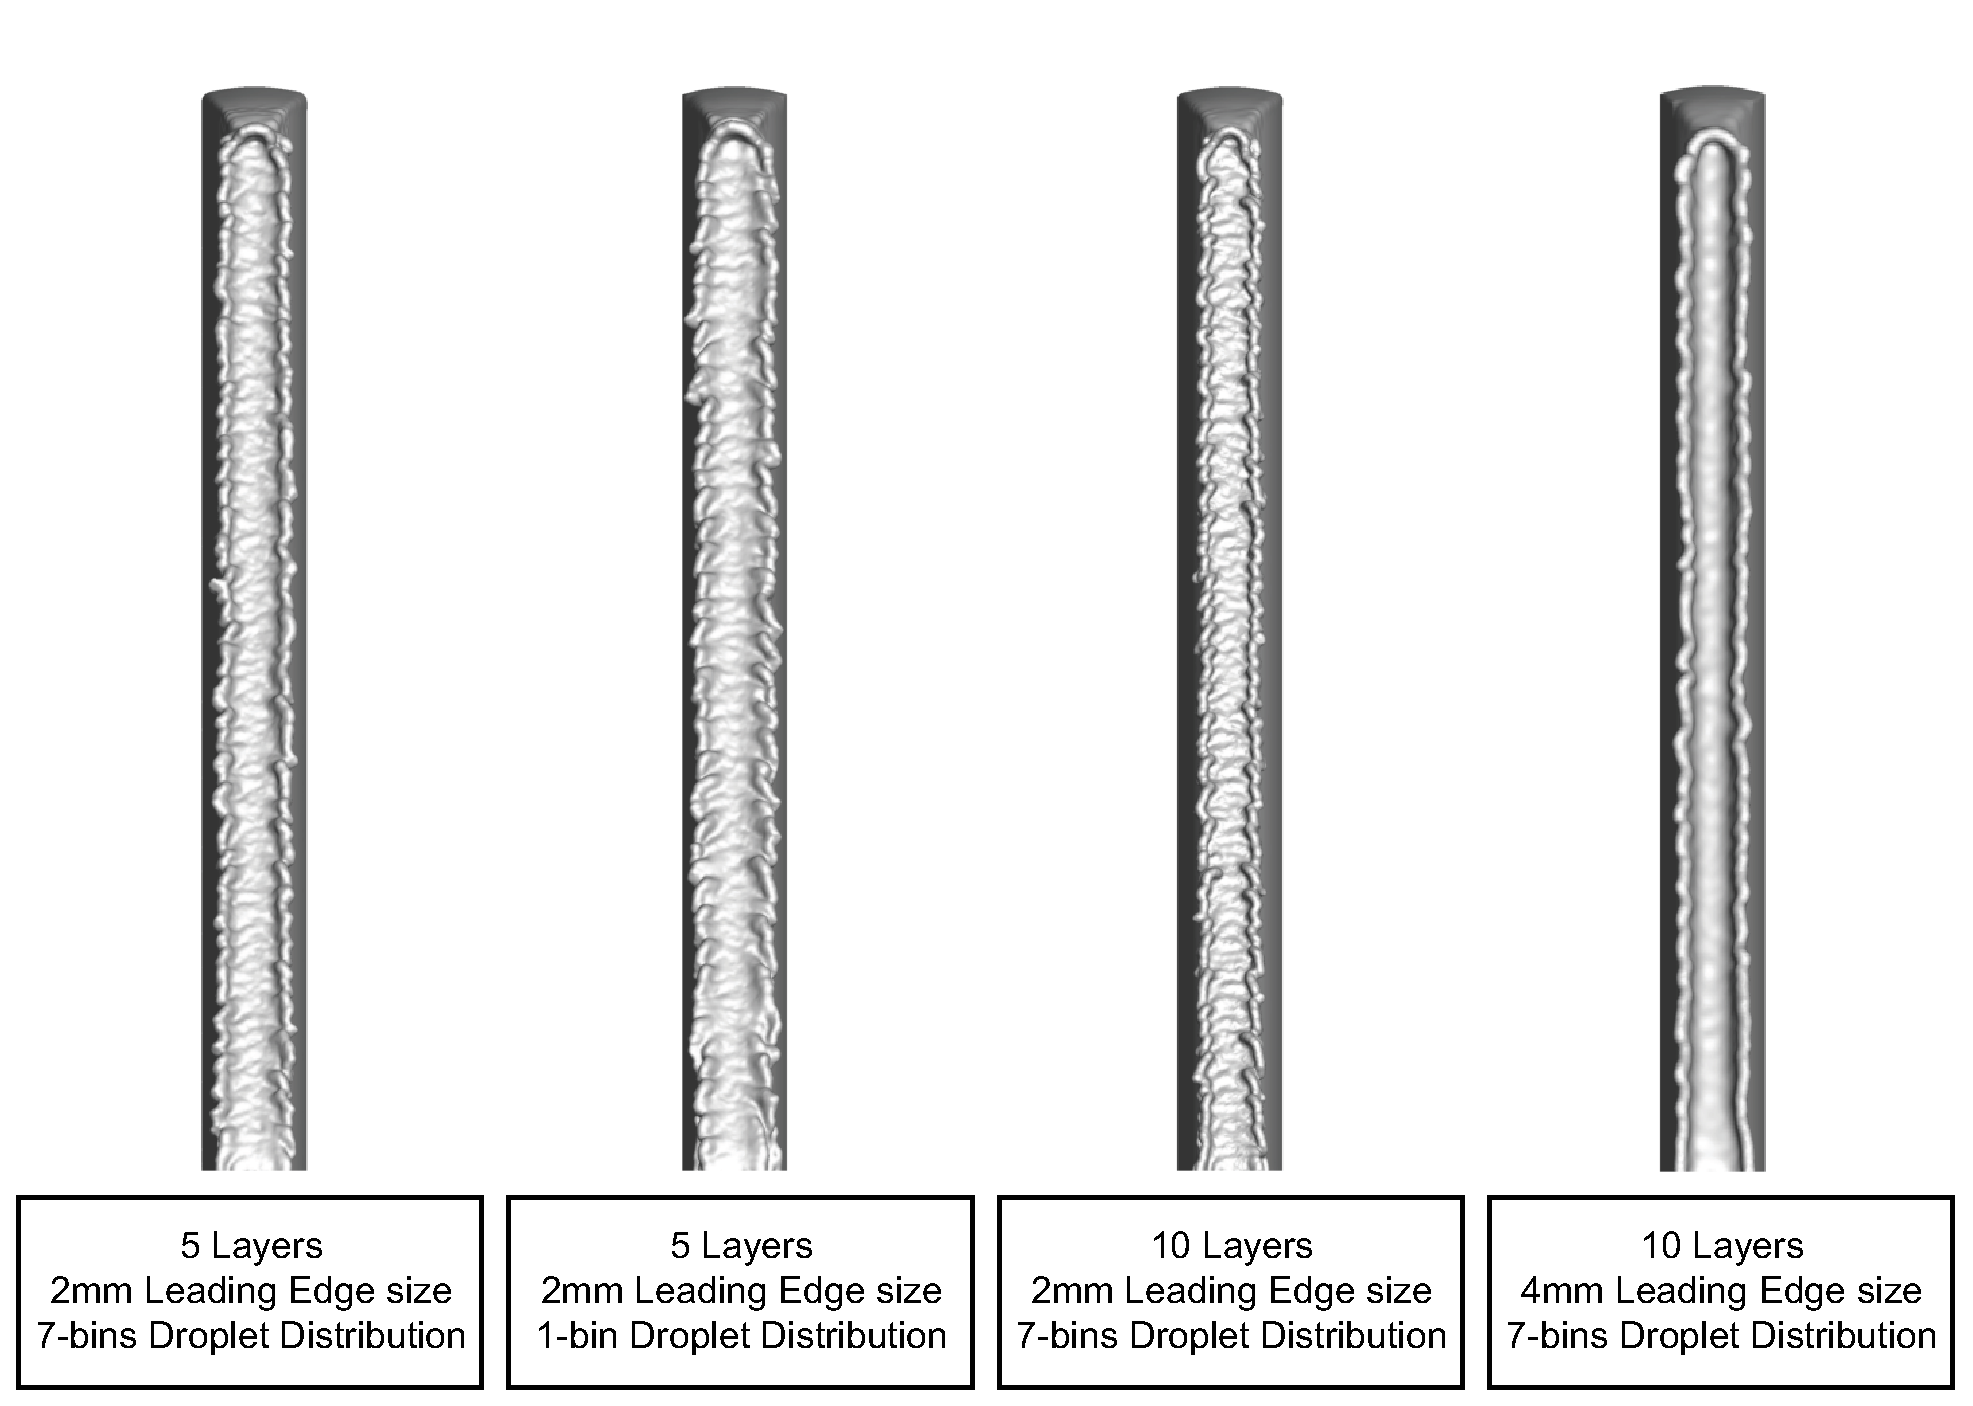
\includegraphics[width=0.8\textwidth]{FIGURES/DISCUSSIONS/3D_ICE_SHAPES.eps}
    \caption{3D level-set ice shapes obtained for different numerical and physical configurations.}
    \label{fig:levelset_parametric_shapes}
\end{figure}

The level-set formulation nevertheless introduces a considerably more elaborate geometry-evolution procedure. Rather than directly displacing the surface mesh, the ice--air interface is represented implicitly as the zero contour of a level-set function defined over an auxiliary volume mesh. Each geometry update therefore requires the construction or adaptation of this volume mesh, initialization of the signed-distance field, propagation of the required surface quantities into the volume, advection of the level-set field, and extraction of the updated zero-level-set surface. These additional operations increase both the computational cost and the complexity of setting up a simulation compared with direct algebraic displacement. Much of this workflow can, however, be automated, such that the additional complexity does not necessarily translate into a comparable increase in user intervention.

% \subsection{Body-Fitted and Immersed-Boundary Approaches}

% As CFD applications are extended toward increasingly complex geometrical configurations, mesh generation can represent a substantial portion of the overall simulation workflow. Generating a computational mesh around a complex geometry is generally straightforward, but obtaining a high-quality body-fitted mesh with adequate near-wall resolution, controlled element quality, and appropriate refinement in regions of interest can require significant user expertise and preparation time. This difficulty becomes particularly important for applications involving evolving geometries, such as ice accretion, where the computational domain may need to be remeshed repeatedly as the ice surface develops. Immersed-boundary methods provide an attractive alternative by relaxing the requirement that the volume mesh conform explicitly to the solid surface.

% In a body-fitted formulation, the computational mesh conforms to the geometry and can therefore provide the near-wall resolution required to capture the boundary layer and other near-wall flow features. This remains an important advantage for aerodynamic and icing calculations, for which quantities such as wall shear stress and heat transfer depend strongly on the near-wall solution. The corresponding disadvantage is the effort required to generate and maintain a high-quality mesh, particularly as the geometry becomes increasingly complex. During multilayer ice accretion, each geometry update may require surface processing followed by regeneration or deformation of the surrounding volume mesh. The robustness of the complete simulation can consequently become dependent on the ability of the meshing procedure to accommodate increasingly irregular ice geometries.

% Immersed-boundary methods shift this difficulty from geometry-conforming mesh generation toward the numerical treatment and spatial resolution of the immersed interface. Since the solid geometry is embedded within a non-conforming background mesh, comparatively regular Cartesian or Cartesian-like grids can be generated with substantially less dependence on the complexity of the surface geometry. This considerably simplifies the treatment of complex and evolving surfaces and eliminates the requirement to regenerate a complete body-fitted volume mesh following every ice-accretion step. The simplicity of the underlying mesh does not, however, remove the need for sufficient spatial resolution near the immersed surface. Accurate representation of the geometry and reconstruction of the near-wall flow quantities still require sufficiently small cells in the vicinity of the interface. Consequently, achieving the required near-surface resolution with an immersed-boundary mesh can require substantially more elements than an equivalent body-fitted discretization.

% This consideration is particularly important for ice accretion. Although an immersed-boundary formulation allows the updated ice geometry to be introduced without regenerating the complete volume mesh, the original background grid must remain sufficiently refined around the continuously evolving ice surface. A mesh designed only around the clean configuration may therefore become inadequate as the ice grows outside the initially refined region. One possible solution is to prescribe a sufficiently large refined region around all locations in which ice growth is expected. This approach is simple and was adopted in the present implementation, but can result in a substantial increase in the total number of computational cells because fine resolution is retained in regions where it may never be required.

% In Chapter~\ref{sec:ibmArticle}, the required near-surface resolution was achieved by prescribing a sufficiently large refined region encompassing either the experimental ice shape or the predicted single-layer ice shape, with an additional margin to accommodate the expected geometry evolution, as illustrated in Figure~\ref{fig:ibm_refined_region}. While suitable for the cases considered, this approach is not practical for general ice-accretion simulations, since it requires prior knowledge or an estimate of the expected ice geometry to prescribe the extent of the refined region.

% \begin{figure}[htbp]
% \centering
% \includegraphics[width=0.6\textwidth]
% {FIGURES/DISCUSSIONS/NACA0012_AMR.png}
% \caption{Example of the prescribed refined region surrounding the NACA0012 geometry and the anticipated ice-accretion region.}
% \label{fig:ibm_refined_region}
% \end{figure}

% Adaptive mesh refinement provides a more general solution to this limitation. Rather than maintaining a fine region surrounding all possible ice geometries, the background mesh can be progressively refined in the vicinity of the evolving immersed interface. The computational resolution can therefore follow the ice geometry as the accretion develops while coarser cells are retained away from the regions of interest. Such an approach considerably improves the practical applicability of immersed-boundary methods for multilayer icing, but requires efficient mesh-adaptation algorithms and data structures capable of dynamically refining and coarsening the background mesh. This represents an important computational challenge, since the adaptation procedure must remain sufficiently efficient to preserve the advantage of the immersed-boundary approach over repeated body-fitted volume-mesh generation.

% The need for efficient adaptive refinement further illustrates the trade-off between body-fitted and immersed-boundary approaches. Body-fitted meshes provide direct control of the near-wall resolution and remain particularly attractive when a high-quality mesh can be generated reliably for the geometry of interest. Their principal limitation for multilayer icing is the repeated mesh-generation problem associated with increasingly complex ice surfaces. Immersed-boundary methods largely remove this dependency on geometry-conforming volume remeshing and consequently offer considerable flexibility for complex and evolving ice geometries, but shift the meshing challenge toward maintaining sufficient local resolution around the evolving interface. Without adaptive refinement, this requirement can lead to prohibitively large background meshes. Consequently, combining an immersed-boundary formulation with efficient adaptive mesh refinement is an important component of a scalable framework for complex multilayer ice-accretion simulations.

\subsection{Body-Fitted and Immersed-Boundary Approaches}

As CFD applications are extended toward increasingly complex geometrical configurations, mesh generation can represent a substantial portion of the overall simulation workflow. While generating a computational mesh around a complex geometry is generally straightforward, obtaining a high-quality body-fitted mesh with adequate near-wall resolution and controlled element quality can require significant effort. This difficulty becomes particularly important for applications involving evolving geometries, such as ice accretion, where the computational mesh must accommodate increasingly complex ice surfaces over successive accretion layers.

Body-fitted meshes provide direct control of the near-wall resolution and are well suited to aerodynamic and icing calculations, for which wall shear stress and heat transfer depend strongly on the near-wall solution. Their main limitation for multilayer ice accretion is the need to maintain a high-quality geometry-conforming mesh as the ice surface evolves. As increasingly complex ice features develop, repeated deformation or regeneration of the volume mesh can therefore become a significant constraint on the robustness of the complete simulation.

Immersed-boundary methods alleviate this constraint by embedding the evolving geometry within a non-conforming background mesh, thereby avoiding repeated generation of a body-fitted RANS mesh. This flexibility comes at the expense of the spatial resolution required near the immersed interface. Accurate representation of the geometry and reconstruction of near-wall quantities require sufficiently small cells around the surface, and the background mesh must remain adequately refined as the ice grows away from the clean geometry.

In Chapter~\ref{sec:ibmArticle}, this requirement was addressed by prescribing a sufficiently large refined region around the anticipated ice-accretion region, as illustrated in Figure~\ref{fig:ibm_refined_region}. While suitable for the cases considered, this approach requires prior knowledge or an estimate of the expected ice geometry and can introduce unnecessary cells in regions where fine resolution is ultimately not required.

\begin{figure}[htbp]
\centering
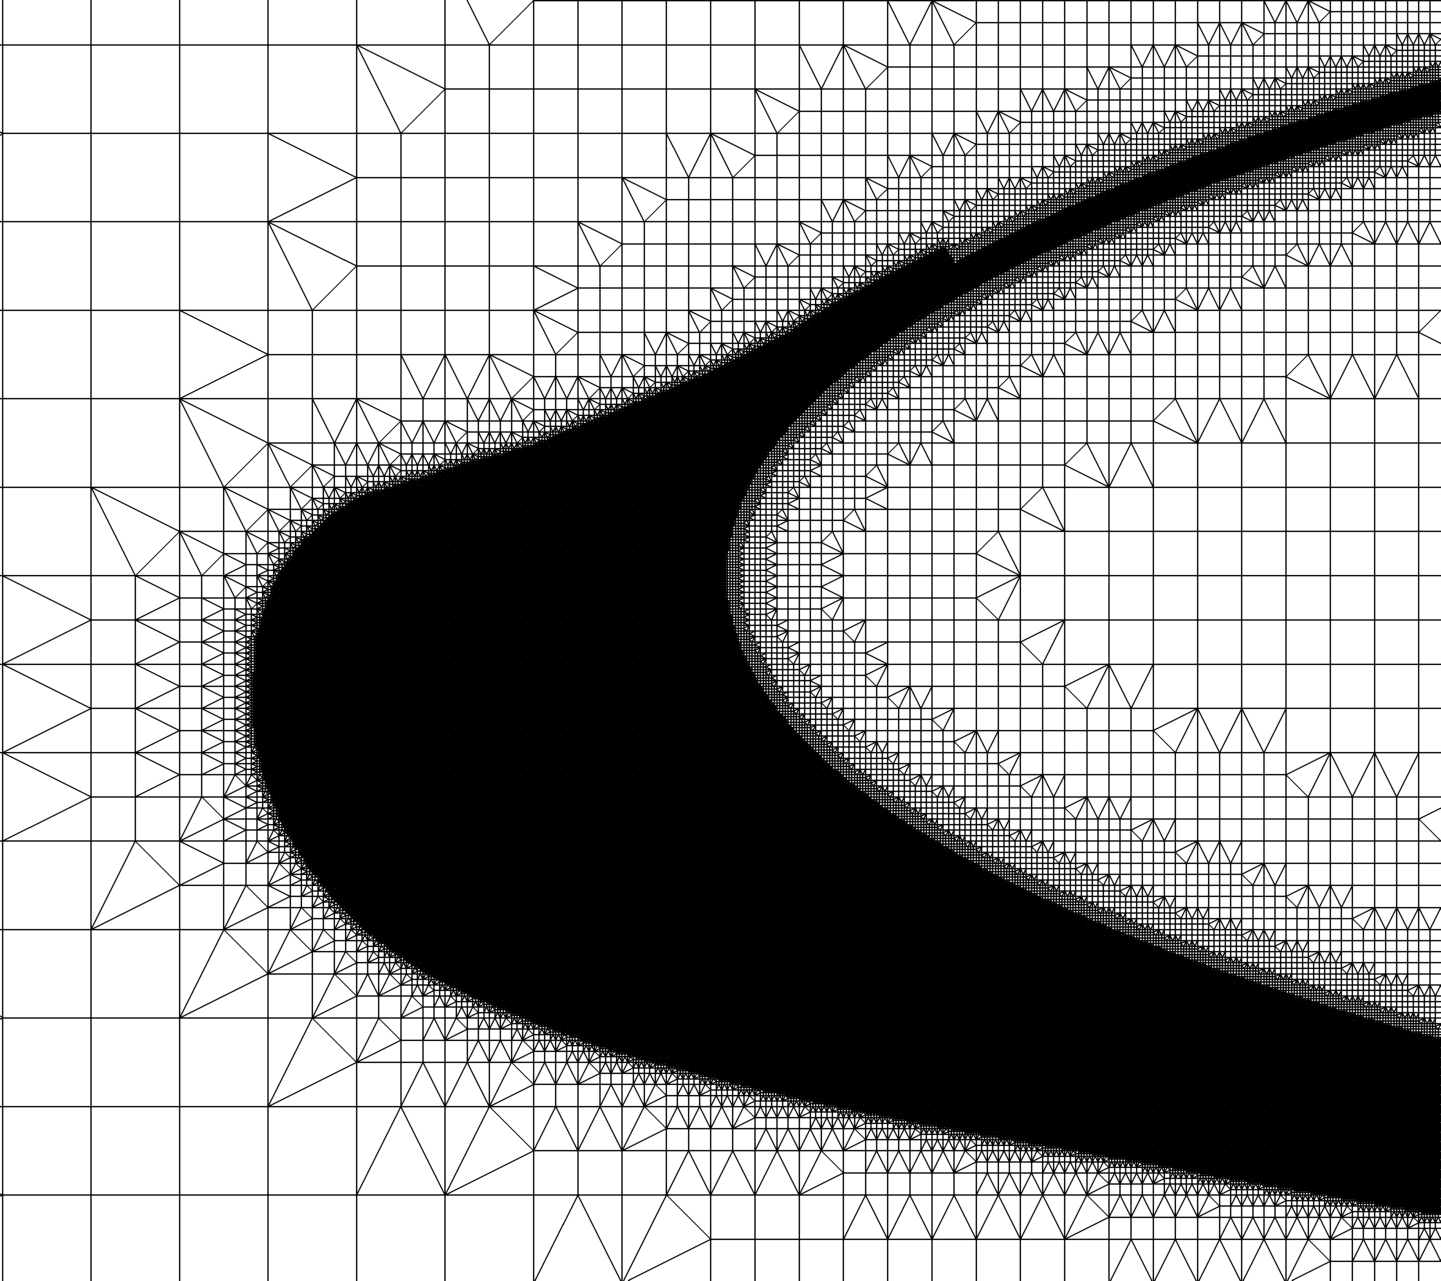
\includegraphics[width=0.5\textwidth]
{FIGURES/DISCUSSIONS/NACA0012_AMR.png}
\caption{Example of the prescribed refined region surrounding the NACA0012 geometry and the anticipated ice-accretion region.}
\label{fig:ibm_refined_region}
\end{figure}

Adaptive mesh refinement provides a more general solution by allowing the background mesh to follow the evolving immersed interface while retaining coarser cells elsewhere. Combining immersed-boundary methods with efficient adaptive refinement would therefore preserve their principal advantage for multilayer icing---avoiding repeated body-fitted volume-mesh generation---without requiring a large predefined region of fine resolution. The main challenge is to perform this adaptation efficiently enough that its computational cost does not offset the advantages of the immersed-boundary approach.